\documentclass[11pt]{article}
\usepackage[margin=19mm]{geometry}
\usepackage[T1]{fontenc}
\usepackage{lmodern}
\usepackage{xcolor,tikz}
\usetikzlibrary{arrows.meta,positioning,calc}
\usepackage{microtype}
\usepackage{fancyhdr}
\pagestyle{fancy}\fancyhf{}\fancyfoot[C]{\thepage}\renewcommand{\headrulewidth}{0pt}
\setlength{\parindent}{0pt}\setlength{\parskip}{7pt}
\tikzset{box/.style={draw=black!55,rounded corners=3pt,align=center,text width=40mm,minimum height=13mm,inner sep=4pt,font=\small},analysis/.style={box,fill=green!12},issue/.style={box,fill=orange!17},arrow/.style={-{Latex[length=2mm]},draw=black!70}}
\begin{document}
{\LARGE Current version}\hfill{\small Review copy · 29 September 2026}

{\large Observability branch}

{\small This reproduces the current branch's labels and connections, with its layout simplified for comparison. Other branches are omitted.}

\begin{center}
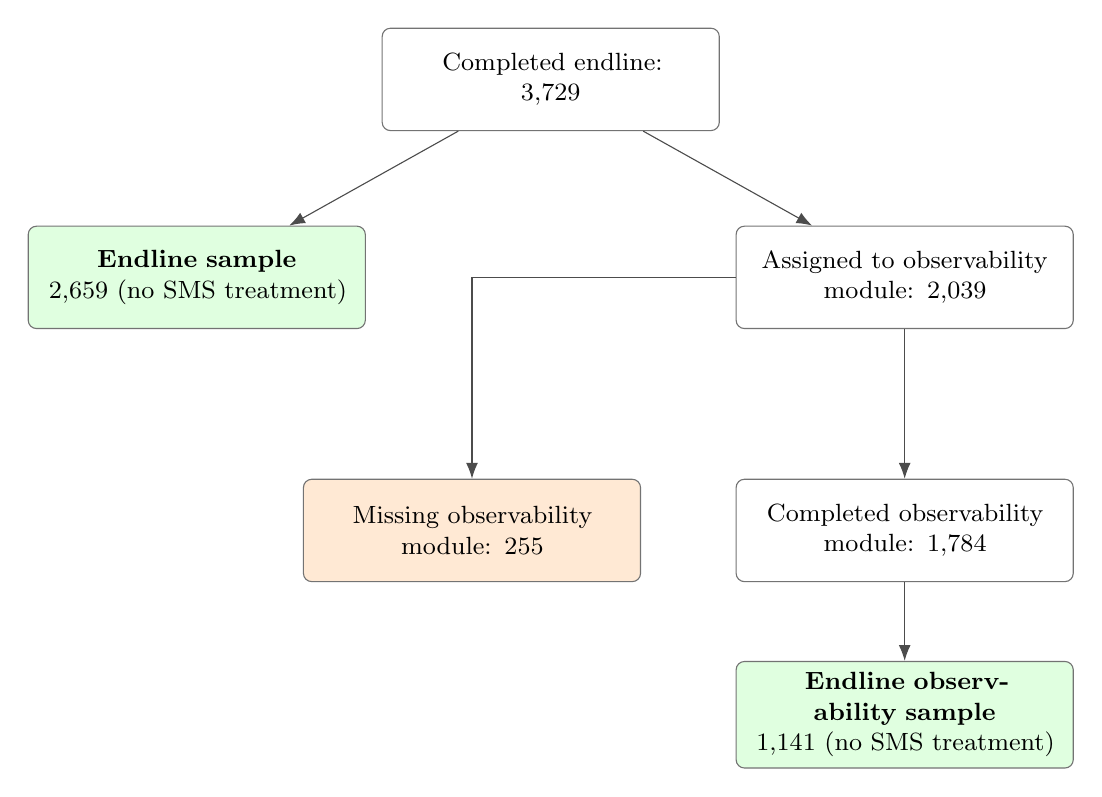
\begin{tikzpicture}[node distance=10mm and 12mm]
\node[box] (full) {Completed endline:\\3,729};
\node[analysis,below left=12mm and 2mm of full] (nosms) {\textbf{Endline sample}\\2,659 (no SMS treatment)};
\node[box,below right=12mm and 2mm of full] (assigned) {Assigned to observability\\module: 2,039};
\node[box,below=19mm of assigned] (complete) {Completed observability\\module: 1,784};
\node[issue,left=12mm of complete] (missing) {Missing observability\\module: 255};
\node[analysis,below=of complete] (sample) {\textbf{Endline observability sample}\\1,141 (no SMS treatment)};
\draw[arrow] (full) -- (nosms);\draw[arrow] (full) -- (assigned);
\draw[arrow] (assigned) -- (complete);\draw[arrow] (assigned.west) -| (missing.north);
\draw[arrow] (complete) -- (sample);
\end{tikzpicture}
\end{center}

{\large Accompanying paragraph — original}

The endline survey generates several additional measures used throughout the analysis. First, 2,039 endline respondents were assigned to an observability module eliciting knowledge of peers' deworming take-up. Of these, 1,784 completed the module and 255 have missing observability module data due to a programming error, discussed in Section [sample balance]. After excluding adults enrolled in SMS treatments, the Endline observability sample contains 1,141 respondents.

{\large Figure notes — original}

{\small\textit{Notes:} Green boxes denote analysis samples used in the main text. The administrative take-up data combine individuals drawn from the baseline roster and the enrolled SMS and no-SMS monitoring rosters, deduplicated across rosters. Because these rosters were drawn independently from the census, individuals may appear in more than one roster before deduplication. The main distance and item/signal analyses exclude adults enrolled in the SMS treatments, which are analyzed separately.}

\newpage
{\LARGE Proposed version}\hfill{\small For review; not applied}

{\large Observability branch}

{\small Branch directly from the existing no-SMS endline sample. Show the sample restrictions on the arrow; keep intermediate counts in the paragraph.}

\begin{center}
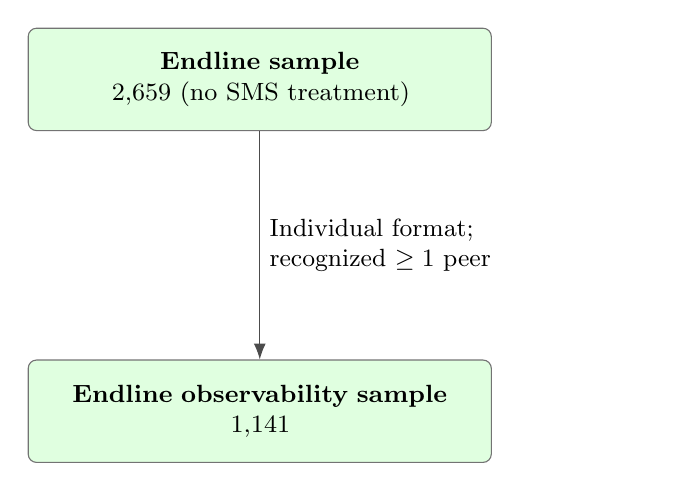
\begin{tikzpicture}[node distance=29mm]
\node[analysis,text width=56mm] (nosms) {\textbf{Endline sample}\\2,659 (no SMS treatment)};
\node[analysis,text width=56mm,below=of nosms] (sample) {\textbf{Endline observability sample}\\1,141};
\draw[arrow] (nosms) -- node[right,font=\small,align=left,text width=49mm] {Individual format;\\recognized $\geq 1$ peer} (sample);
\end{tikzpicture}
\end{center}

{\large Accompanying paragraph — suggested}

Among the 2,659 no-SMS endline respondents, 1,204 completed the individual knowledge format and 1,203 completed the paired format; 252 lacked knowledge-module data. Of those completing the individual format, 1,141 recognized at least one peer and form the Endline observability sample.

{\large Figure notes}

Retain the existing figure notes. The simulation explanation remains in the missingness-table notes and main-text footnote.

\vfill
{\small\textit{Separate unresolved count:} The manuscript reports 3,729 completed endline surveys; the saved clean endline dataset contains 3,678 respondents. This proposal reconciles the verified no-SMS observability branch only. It does not resolve that upstream difference.}
\end{document}
